\documentclass[12pt, a4paper]{report}
\usepackage[utf8]{inputenc}
\usepackage{blindtext}
\usepackage{float}
\usepackage{graphicx}
\usepackage{siunitx}
\usepackage{geometry}

\newgeometry{
    top=1in,
    bottom=1in,
    inner=1in,
    outer=1in,
    paper=a4paper
}

\title{\textbf{\Large{NUTS CubeSat}}}
\author{Ali Malik}
\date{March 05, 2022}

\begin{document}

\maketitle

\tableofcontents
\newpage
\listoffigures


% \addcontentsline{toc}{chapter}{\textbf{Background}}
\chapter{Background}

The NTNU Test Satellite (NUTS) project is a student satellite project at the Norwegian University of Science and Technology (NTNU). The project is part of Norway's national student satellite program, which is overall manager by the Norwegian Centre for Space relate Education (NAROM)\cite{overview}. The initial goal of the NUTS project was to design, develop, test, launch, and operate a CubeSat by 2014, this target date was delayed to sometime in 2016, and since then this launch date has bounced around from 2017 and later. With no clear launch date in sight, the project slowly evolved into Orbit NTNU, a non-profit student organization. This report aims to analyze the initial design for the NUTS satellite.

NTNU has experimented with CubeSats in the past, specifically, the nCube in the early 2000s. nCube-1 and nCube-2 were both developed in the early 2000s and  launched in mid 2006 and late 2005, respectively. Unfortunately, radio contact with nCube-2 was never achieved, but NTNU was able to track it down via radar. nCube-1 was launched but due to a problem with the second stage of the rocket causing a launch abort. Both satellites were single CubeSats (1U) with the following dimensions, \(10 \unit{\centi\meter} \times 10 \unit{\centi\meter} \times 10 \unit{\centi\meter}\) and weighed around \(1 \unit{\kilo\gram}\), which is in accordance with the CubeSat Standard for a 1U CubeSat \cite{cubesat_standard}.

The goal of this report is to analyze the CubeSat, specifically the hardware architecture, the modules, and subsystems.

% \addcontentsline{toc}{chapter}{\textbf{Design}}
\chapter{Design}

% \addcontentsline{toc}{section}{\textit{Overall Design}}
\section{Overall Design}

The NUTS CubeSat was created in to allow multidisciplinary students the ability to gain real world application knowledge of designing, manufacture, and launching a double CubeSat \cite{power_distribution}. The NUTS was a Low-Earth Orbit (LEO) nano-satellite measuring roughly \(10 \unit{\centi\meter} \times 10 \unit{\centi\meter} \times 20 \unit{\centi\meter}\) and weighed less than \(2.66 \unit{\kilo\gram}\) which is in accordance with the CubeSat Standard for a 2U CubeSat \cite{power_distribution}\cite{cubesat_standard}.

Figure~\ref{fig:overall_design} specifies the over-arching design for the CubeSat highlighting the main sub-systems and components within the NUTS project. 

\begin{figure}[H]
    \centering
    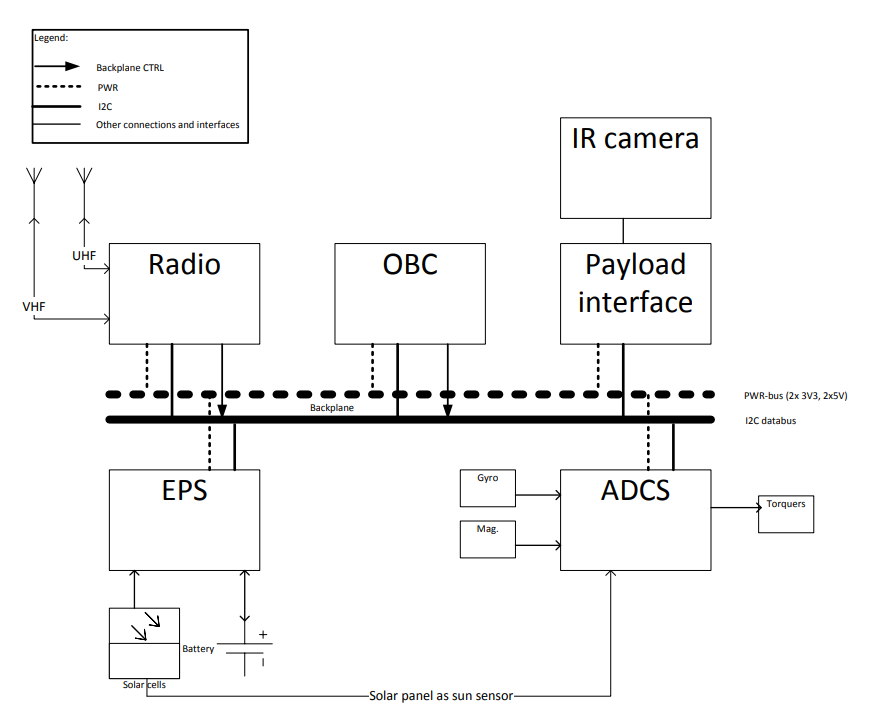
\includegraphics[width=300pt]{images/nuts_design.PNG}
    \caption{A very simple overview of the design for the NUTS CubeSat\cite{overview}}
    \label{fig:overall_design}
\end{figure}

The overall design includes many components such as:

\begin{itemize}
    \item A radio - Communication Subsytem
    \item Electrical Power System (EPS)
    \item Attitude Determination and Control System (ADCS)
    \item On-Board Computer (OBC)
\end{itemize}

The main architecture of the CubeSat is more a distributed systems approach, which means, giving most, if not all, subsystems their own micro-controller (MCU), a common design approach for CubeSats. There is one distinction to be made, the NUTS CubeSat does not utilize the default method of stacking electronic boards to represent modules instead, the NUTS CubeSat implements a common backplane, to be shared with all components, with slots for each subsystem. This design approach comes from the lessons learned from the nCube satellites \cite{overview}. 

Figure~\ref{fig:overall_design_2} shows another version of the same design that was shown in Figure~\ref{fig:overall_design}.

\begin{figure}[H]
    \centering
    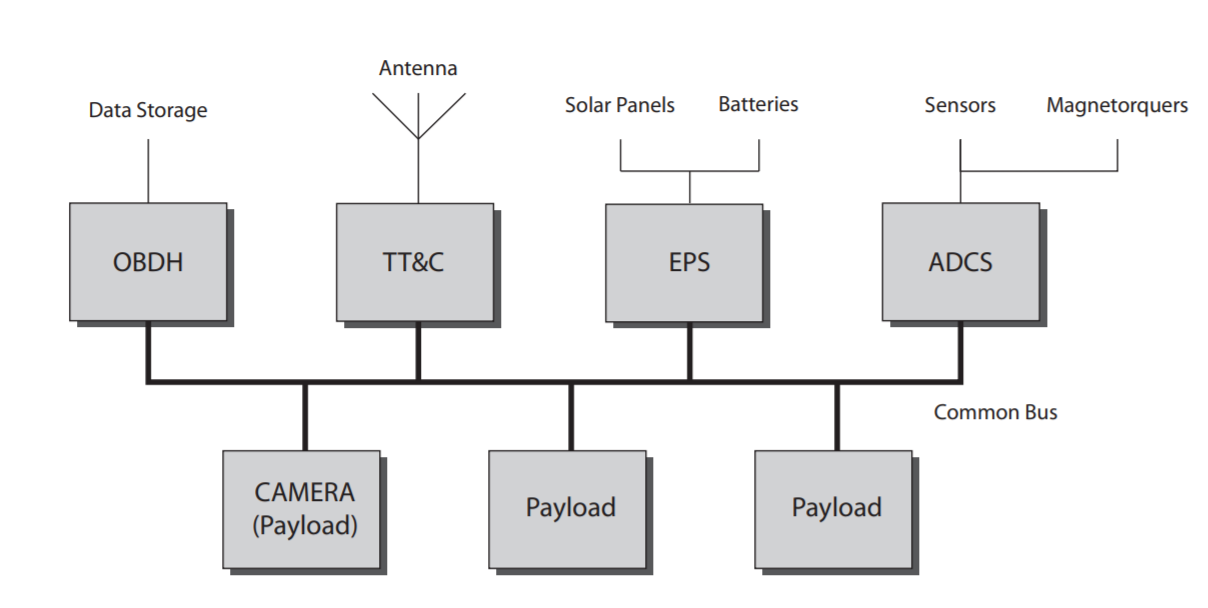
\includegraphics[width=300pt]{images/nuts_design2.PNG}
    \caption{Another version of the design for the NUTS satellite \cite{power_distribution}}
    \label{fig:overall_design_2}
\end{figure}

As observable, some of the major modules shown in this figure that are named differently in Figure~\ref{fig:overall_design} include:

\begin{itemize}
    \item On-Board Data Handling \(\rightarrow\) On-Board Controller
    \item Telemetry, Tracking, and Control (TT\&C) \(\rightarrow\) Radios
\end{itemize}

Figure~\ref{fig:subsystems} highlights the specific components that were used to build the NUTS satellite:

\begin{figure}[H]
    \centering
    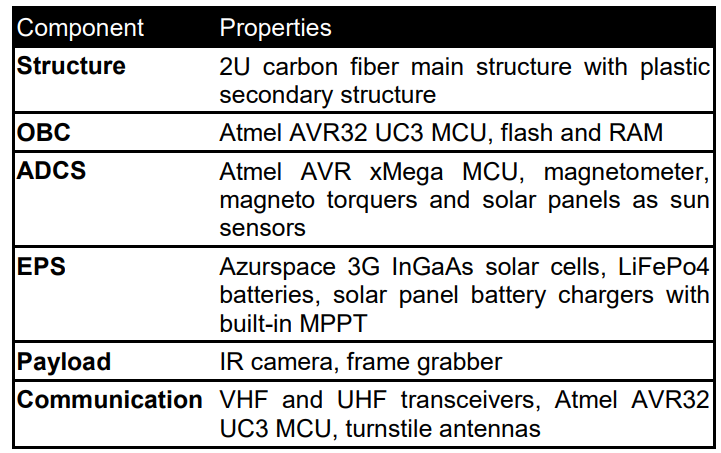
\includegraphics[width=300pt]{images/nuts_subsystems.PNG}
    \caption{Specific Satellite Subsystems\cite{overview}}
    \label{fig:subsystems}
\end{figure}

We'll examine each of these components a bit more in depth in the following subsections. 

% \addcontentsline{toc}{section}{\textit{Structure}}
\section{Structure}

As mentioned in Figure \ref{fig:subsystems}, the main structure of the NUTS CubeSat is made of carbon fiber, which is in complete contrast to normal CubeSat structures \cite{nasa_structure}. Most CubeSats have chassis/frames that are machined from aluminum alloys that provide mounting locations and allow for flexibility in configurations \cite{nasa_structure}. The benefits of carbon fiber as a main structure are:
\begin{itemize}
    \item High strength/stiffness
    \item Corrosion Resistance
    \item Lightweight
    \item Low Coefficient of Thermal Expansion (CTE)
\end{itemize}

Due to the low weight of carbon fiber it makes it possible to decrease the structural weight and allows for more capacity for other modules and the payload. In addition to the main structure being made of carbon fiber, the inner structure is made of a polymer material which will be used to fasten the backplane and the subsystem circuit boards in place. This polymer inner structure can easily be changed and still fit inside the main chassis without problems. Figure \ref{fig:structure} shows the model for the main and inner structures, with solar panels and some electronics mounted:

\begin{figure}[H]
    \centering
    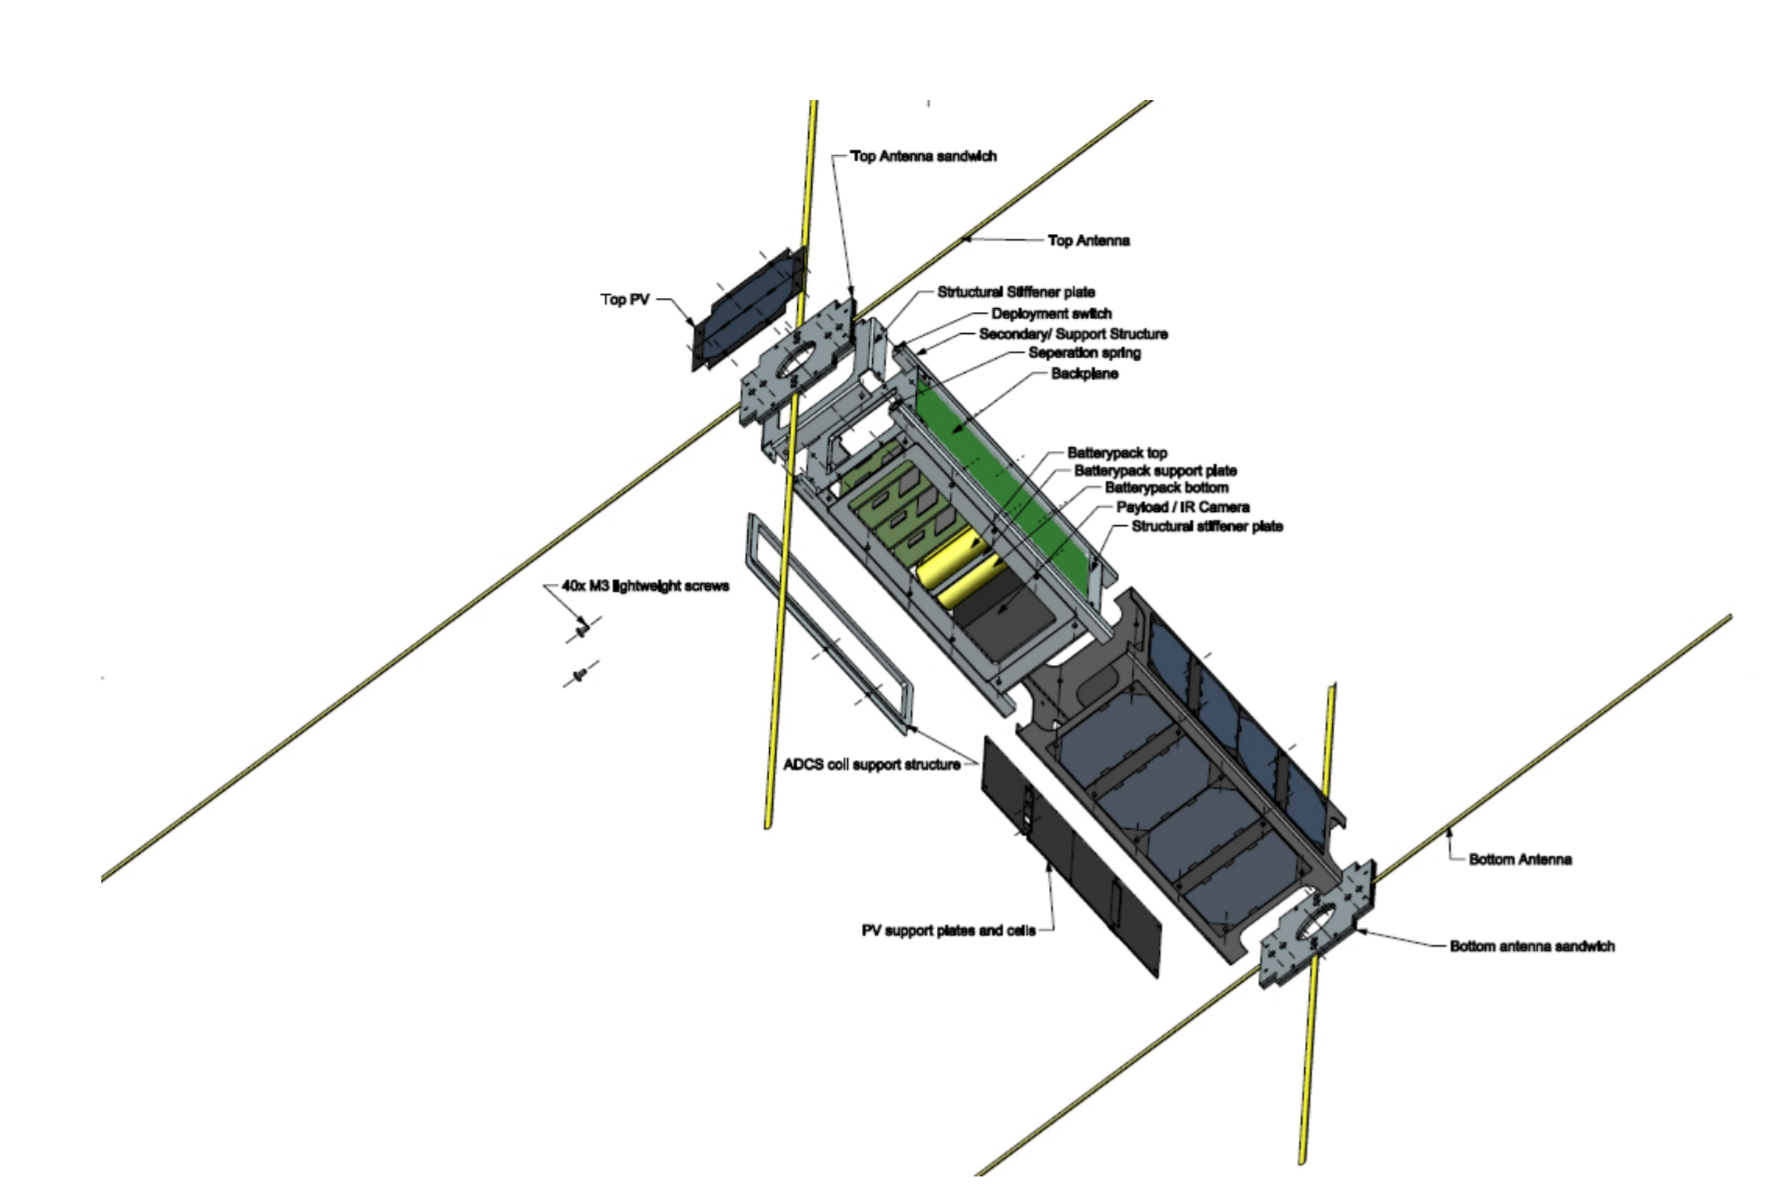
\includegraphics[width=300pt]{images/nuts_structure.PNG}
    \caption{NUTS Physical Structure \cite{overview}}
    \label{fig:structure}
\end{figure}

Using the carbon fiber as the material for the main chassis was a risk because, it's important for the structure to behave similarly to that of commercial-of-the-shelf (COTS) aluminum structures in launch and orbit environments. During the production of the NUTS satellite, the engineers relied on Finite Element Models (FEM) to determine the structural stress and deformation response, these results were made the basis for testing preparations \cite{overview}.

% \addcontentsline{toc}{section}{\textit{Backplane}}
\section{Backplane}

The backplane is the electronic infrastructre within the satellite. A key component, the backplane serves as the both the physical and electrical interconnect between all subsystem modules. The backplane handles problems with power distribution and management. The NUTS backplane also implemented additional features such as important protection and monitoring, and the ability to isolate modules to prevent from shared failure, where one subsystems failure causes another failure \cite{power_distribution}. 

Each subsystem will have its own slot that connects it to the backplane. The backplane provides both, a double \(3.3 \unit{\volt}\) and a double \(5 \unit{\volt}\) bus. The backplane also provides a connection into the main data bus, which is an I\textsuperscript{2}C bus. One of the most important design decision was increasing the reliability of the satellite bus. In that effort, the power supply into two separated buses. This decision increases redundancy, as well as, reliability in the system. In the case that a single bus is shorted, the other bus remains fully functional, never leaving the subsystems without power \cite{overview}. 

In completion the backplane provides:

\begin{itemize}
    \item Redundant \(3.3 \unit{\volt}\) and \(5 \unit{\volt}\) power supply buses.
    \item Adjustable \(2.5 \unit{\milli\ampere} - 1.5 \unit{\ampere}\) current limited power switched with auto-retry functionality \cite{power_distribution}
    \item Voltage and current monitoring and outputting that data on the I\textsuperscript{2}C bus
\end{itemize}

Figure~\ref{fig:nuts_backplane} shows the power distribution module that the backplane will utilize:

\begin{figure}[H]
    \centering
    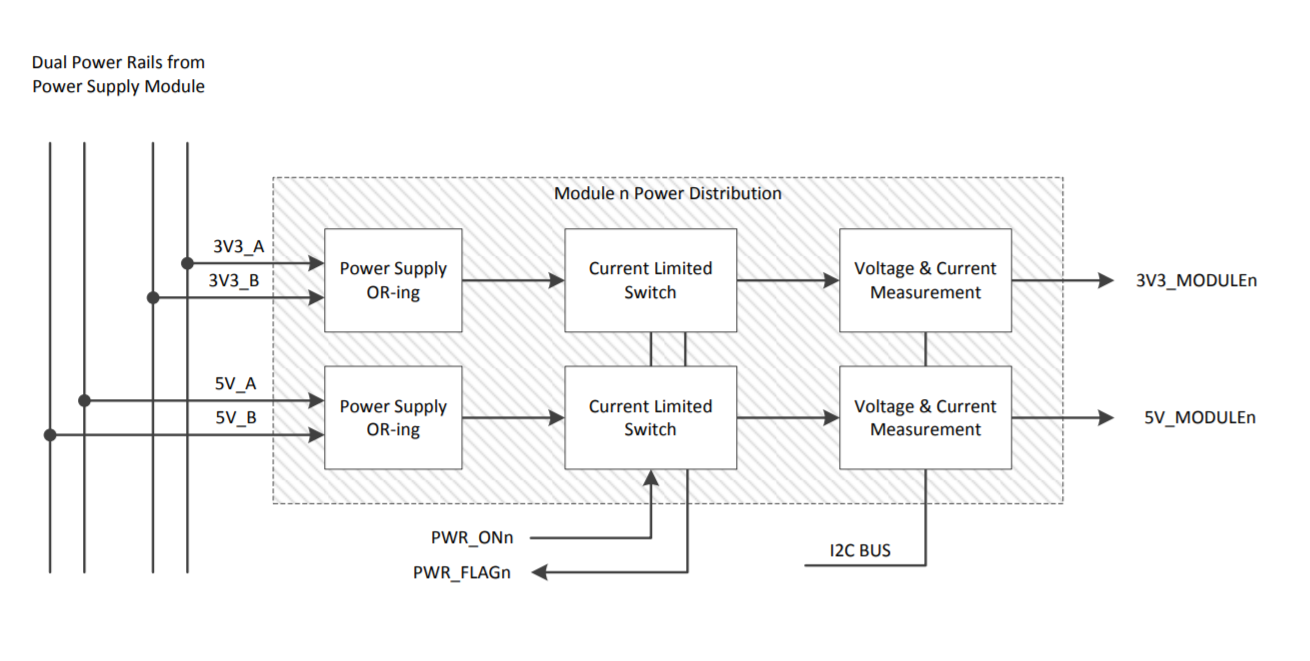
\includegraphics[width=300pt]{images/nuts_backplane2.PNG}
    \caption{NUTS Backplane power module \cite{power_distribution}}
    \label{fig:nuts_backplane}
\end{figure}

The combination of redundant power supplies is done so using a special OR-ing controller, which act as ideal diodes and protect both the secondary power supply as well as the bus in case a power supply fails. The monitoring is realized using high-side shunt resistors with a current sense amplifier to note current \cite{power_distribution}. The power distribution module also include an Analog to Digital Converter (ADC) and an interface to connect to the I\textsuperscript{2}C bus.

Figure~\ref{fig:nuts_backplane_2} shows another view for the backplane:

\begin{figure}[H]
    \centering
    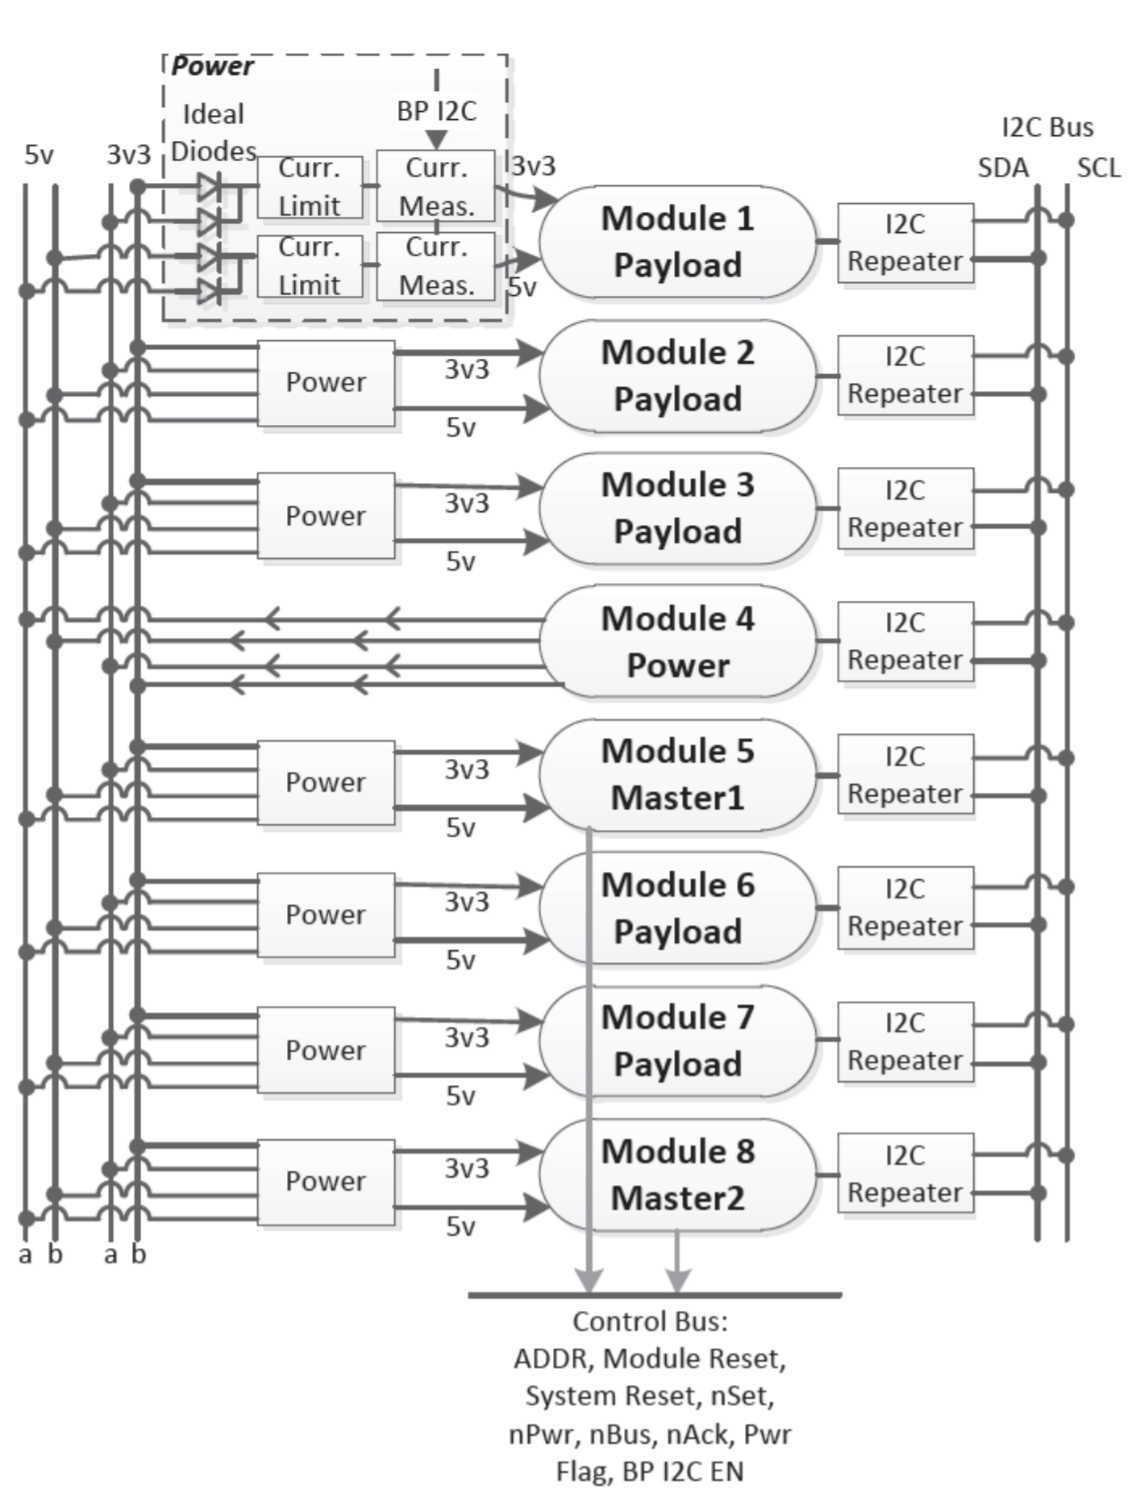
\includegraphics[width=300pt]{images/nuts_backplane.PNG}
    \caption{Overview of NUTS Backplane \cite{overview}}
    \label{fig:nuts_backplane_2}
\end{figure}

Each backplane slot is equipped with control electronics that provide functionality to disconnect the subsystem from the power bus, as well as, isolating the subsystem from the I\textsuperscript{2}C databus. The aforementioned control electronics can be operated by two of the subsystems, the OBC and the communications module. Typically, the OBC will be in charge, but if it fails manual control is possible using the radio link. This design creates some impedance in satellite operations, but it allows for possible satellite control. The backplane also provides communication between subsytems using the CubeSat Space Protocol (CSP) over the I\textsuperscript{2}C bus. CSP is used between the "active" parts of the satellite system internally, as well as, between the satellite and ground station \cite{overview}.

Figure~\ref{fig:backplane_pcb} shows the final backplane PCB.

\begin{figure}[H]
    \centering
    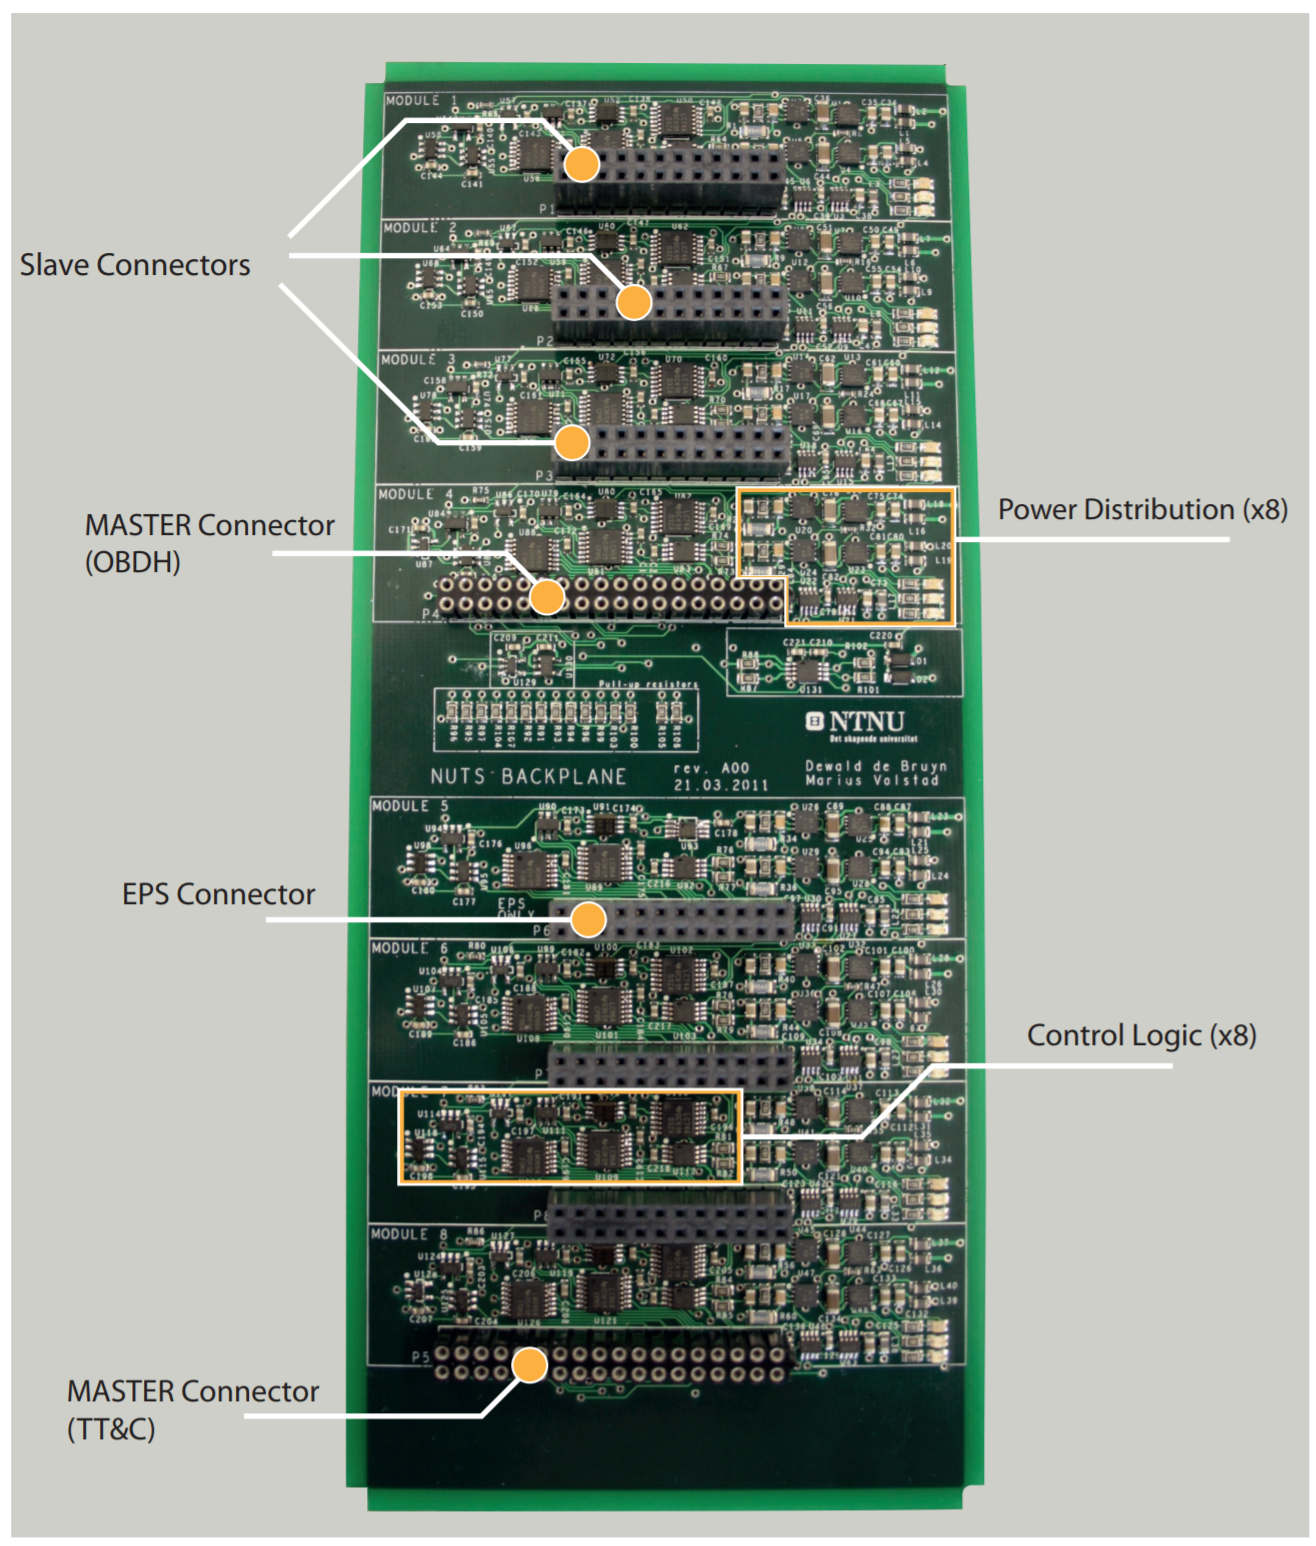
\includegraphics[width=300pt]{images/nuts_backplane_final.PNG}
    \caption{The Final Backplane PCB \cite{power_distribution}}
    \label{fig:backplane_pcb}
\end{figure}

% \addcontentsline{toc}{section}{\textit{Electrical Power System (EPS)}}
\section{Electrical Power System (EPS)}

In combination with the backplane, the Electrical Power System (EPS) module are responsible for the power management for the entire satellite. The backplane is responsible for distributing the power and protecting the subsystems from power-related issues, the EPS is responsible for providing that power. The providing of power includes everything from converting power radiated from the sun, battery charging and monitoring, and regulating the voltage of the bus in general \cite{power_distribution}.

The EPS has the following purposes \cite{power_distribution}:

\begin{itemize}
    \item To supply \(2 \times 3.3 \unit{\volt}\) power rails to the backplane.
    \item To supply \(2 \times 5 \unit{\volt}\) power rails to the backplane.
    \item Charge batteries using power provided by solar cells.
    \item Prevent batteries from over-charge and over-discharge.
    \item To provide telemetry data about battery state-of-charge and available power from solar panels.
\end{itemize}

Since the EPS is responsible for charging the batteries using the solar cells, it's important recognize that the current draw from the solar panels should be controlled in some way. The efficiency of the solar panels truly depends on where on the Solar Cell IV Curve the cells are being operated on. Figure~\ref{fig:solar_iv} shows the I-V Curve for a Solar Cell. The efficiency of the solar cells take a hit depending on how much current is drawn, too much or too little current drawn could lead to an inefficient system. To combat this, maximum power point tracking (MPTT) was implemented to get the most power out of the cells and in the most efficient manner \cite{power_distribution}. 

\begin{figure}[H]
    \centering
    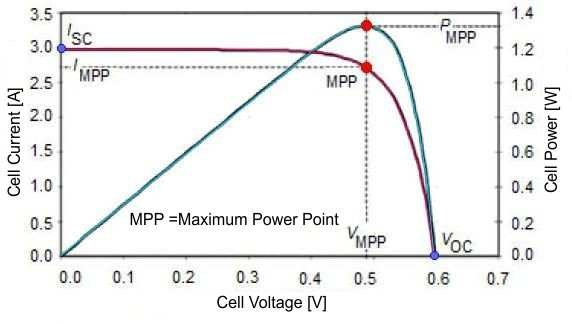
\includegraphics[width=300pt]{images/solar_iv.png}
    \caption{Characteristic Curve of a Solar Cell \cite{solar_cell}}
    \label{fig:solar_iv}
\end{figure}

In addition to the charging of the batteries, the EPS is responsible for monitoring and controlling energy consumption in the satellite. This includes tasks such as; turning modules on/off depending on energy availability and module health status \cite{overview}. Below are two architecture diagrams for the EPS:

\begin{figure}[H]
    \centering
    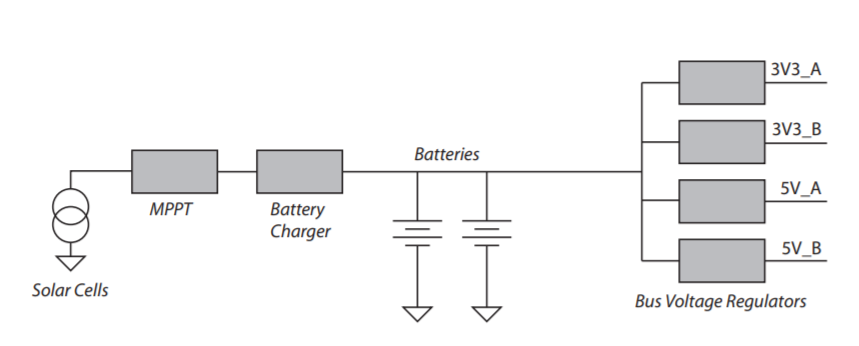
\includegraphics[width=300pt]{images/eps_1.PNG}
    \caption{Overview of EPS Architecture \cite{power_distribution}}
    \label{fig:eps_1}
\end{figure}

\begin{figure}[H]
    \centering
    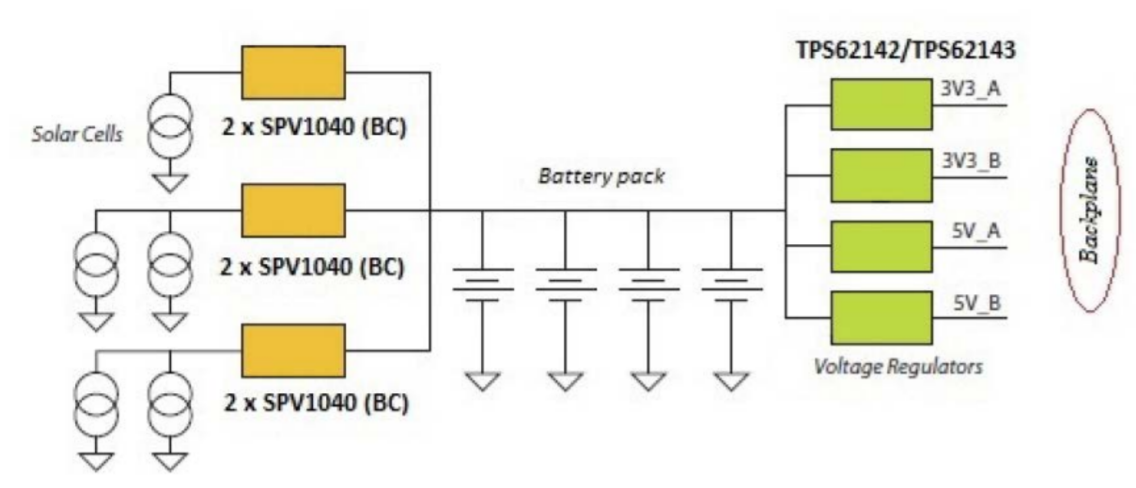
\includegraphics[width=300pt]{images/eps_2.PNG}
    \caption{Another view of the EPS Architecture \cite{overview}}
    \label{fig:eps_2}
\end{figure}

% \addcontentsline{toc}{section}{\textit{Attitude Determination and Control System (ADCS)}}
\section{Attitude Determination and Control System (ADCS)}

The Attitude Determination and Control System is a subsystem that's responsible for two key functionalities [NASA\_ADCS]:

\begin{itemize}
    \item \textbf{Attitude Determination}: the process of combining available sensor data with knowledge of spacecraft specific dynamics to provide a unique and accurate solution for the attitude state of a system as a function of time.
    \item \textbf{Attitude Control}: the combination of the prediction of and reaction to a vehicles rotational dynamics.
\end{itemize}

To simplify, the ADCS module's responsibility is two-sided: obtaining estimates for satellite orientation, and to provide de-tumbling and stabilization \cite{power_distribution}. 

In the case of the NUTS satellite, the ADCS is similar to other systems, in that, it employs magnetic torquers in the form of coils wound up inside the frame \cite{overview}. The NUTS satellite uses a gyro, magnetometer, and solar panels as sensors. The gyro provides angular momentum, the magnetometer provides the magnetic induction, and the solar panels are used as sun sensors. Once the orientation data is gathered, it's passed to the attitude controller which uses the magnetic torquers as actuators to stabilize the satellite flight \cite{power_distribution}. Stabilization is a key component, it ensures that the antenna systems and cameras (payload) are pointed in the right direction. In terms of estimator algorithms, the NUTS satellite tested and implemented a few of them including, the Extended Kalman Filter, Extended Quaternion Estimator, and the Nonlinear Observer \cite{overview}. Figure~\ref{fig:adcs} show an overview of the ADCS subsystem:

\begin{figure}[H]
    \centering
    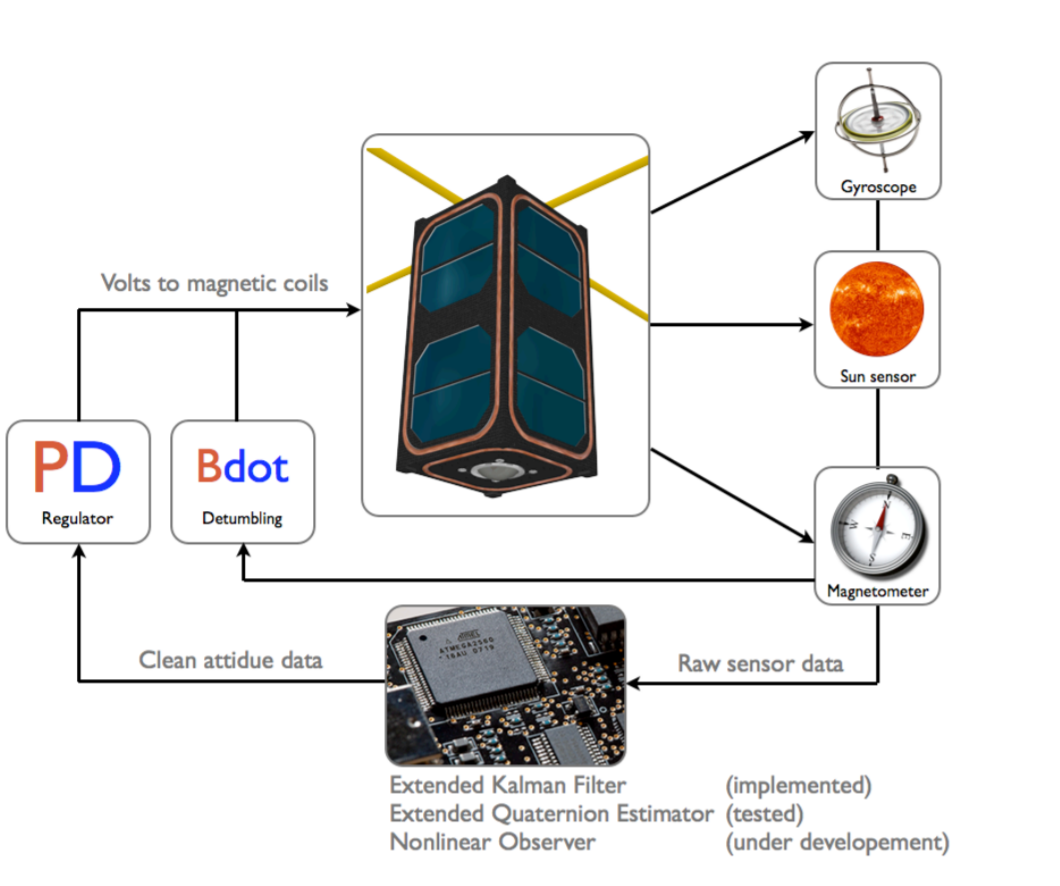
\includegraphics[width=300pt]{images/nuts_adcs.PNG}
    \caption{Overview of the ADCS Subsystem}
    \label{fig:adcs}
\end{figure}

% \addcontentsline{toc}{section}{\textit{On-Board Computer (OBC)}}
\section{On-Board Computer (OBC)}

The On-Board Computer (OBC) is one of the main modules within the NUTS satellite. This module has complete control over the backplane. The OBC is the satellites main controller and contains the main mission computer, as well as, the memory for the software and data storage \cite{overview}\cite{power_distribution}. The OBCs main tasks are to monitor system health, logging flight data, and to issue commands to other modules according to the planned mission. In addition, the OBC is responsible for making decision in case of anomalies and payload data processing \cite{overview}.

The OBC for the NUTS satellite is composed of an Atmel ACR32 UC3 with access to external flash and Random Access Memory (RAM). The OBC runs the FreeRTOS operating system, which is a reliable, lightweight, simply, and very feature rich real-time operating system \cite{freertos}. Figure~\ref{fig:obc} shows an early version of the backplane with the OBC connected:

\begin{figure}[H]
    \centering
    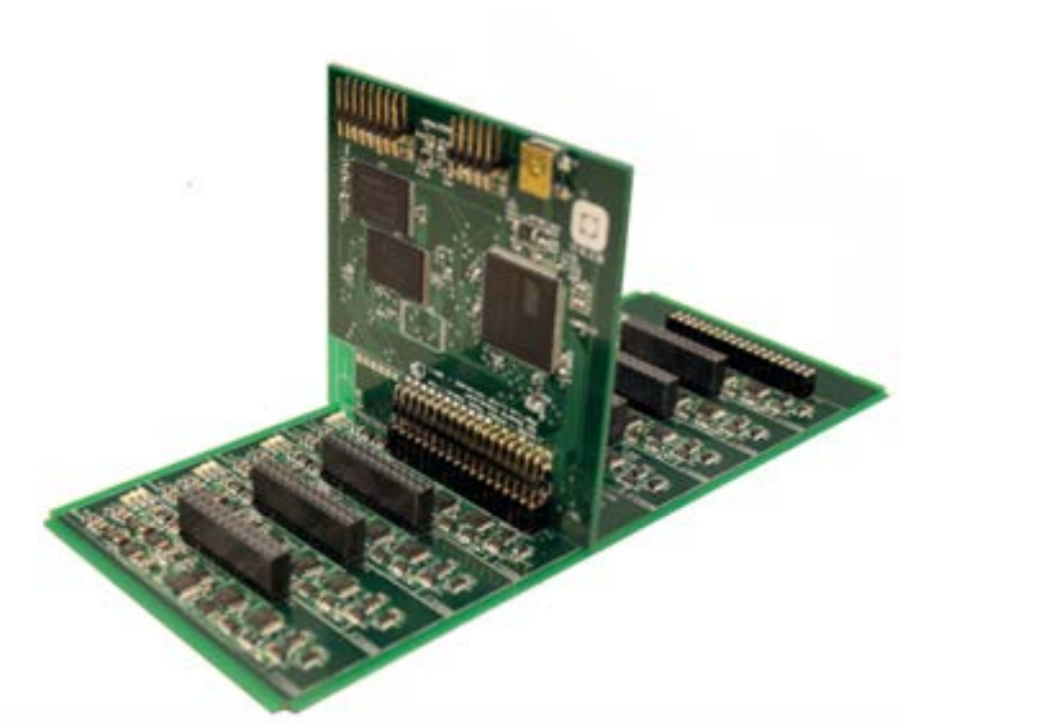
\includegraphics[width=300pt]{images/nuts_obc.PNG}
    \caption{Backplane with the OBC connected \cite{overview}}
    \label{fig:obc}
\end{figure}

An important part of the OBC is the copies of the systems software that's contained within a radiation-tolerant read-only memory (ROM), which allows the restoring of corrupt instruction memories. This allows the system to recover in case of exposure to space radiation like high energy ion radiation, magnetic fields and plasma interactions, which can cause memory corruption, degradation, or permanent damage of components/modules \cite{radiation}.

% \addcontentsline{toc}{section}{\textit{Communication Subsystem}}
\section{Communication Subsystem - Telemetry, Tracking, and Control}

The Telemetry, Tracking, and Control module, TT\&C, along withe OBC is the other main module within the NUTS ecosystem. The communication subsystem is what allows for communication with the satellite, which is an extremely important capability, as loss of communication generally signifies the end of the mission. The onboard radios use integrated transreceivers with the necessary amplifiers. The NUTS satellite utilizes the standard ham radio bands, giving the community access to the data. The NUTS satellite utilizes a circular polarized turnstile antenna which includes both a UHF (\(145 \unit{\mega\hertz}\)) radio and a VHF (\(437 \unit{\mega\hertz}\)) radio\cite{overview}\cite{power_distribution}.

In addition to being able to receive commands from the ground station and sending data back, the communication subsystem also contains a periodic beacon signal, which can be picked up amateur radios around the world. This module, in addition to the OBC, can take complete control of the satellite from the ground station should the OBC fail\cite{power_distribution}.


\section{Payload}

The payload for the NUTS satellite is an infrared (IR) camera that can capture images of short-period gravity waves in the OH airglow layer. The airglow layer is located roughly \(90 \unit{\kilo\meter}\) in the Mesosphere and lower Thermosphere (MLT)\cite{overview}.

Some of the challenges the NUTS team faced were finding suitable cameras that'd meet the mechanical and operational requirements of being able to capture good scientific data under harsh conditions\cite{overview}. In addition, since the camera won't be directly connected to the OBC, another component is required, a frame grabber. 

Another challenge is the fact that the infrared radiation from the airglow layer is only measurable during local night. Which implies that to achieve the best results the camera should be imaging the atmosphere over a certain point on Earth roughly five hours after local sunset\cite{overview}. Another challenge is the limited downlink capacity, even if the captured images aren't large it'll pose a challenge for the downlink. To alleviate and address these concerns, NUTS investigated many compression and smart image processing techniques. 

\section{Conclusion}

In conclusion, the goal of this paper was to identify and examine the design principles and decisions taken to create the NUTS satellite. This paper addressed the following:

\begin{itemize}
    \item Overall Design
    \item The Structure
    \item Backplane and its design and interconnects
    \item EPS and it's responsibilities in the system
    \item ADCS, it's responsibilities in the system, and its implementation
    \item OBC, its capabilities, design decisions, and responsibilities
    \item Communication Subsystems, implementation, and the responsibilities in case of OBC failure
    \item And lastly, we briefly discussed the payload and the mission.
\end{itemize}

Although the NUTS satellite didn't have a successful launch, the work put in by the team did lead to direct successors such as the HYPSO-1, HYPSO-2, SelfieSat-1, Orbit, and the FRAMSAT-1. Not only did the NUTS project lead to more successful successors, it lead to the creation of the Small Satellite Lab within NTNU, which is responsible for strengthening the small satellite and space related activities at NTNU and make them more visible. Overall, the NUTS project wasn't completed but provided the basis for successful launches of many other CubeSats originating from NTNU. 

\bibliographystyle{plain}
\bibliography{ref}

\end{document}
